\documentclass[11pt]{article}
% \usepackage{times}
\usepackage{booktabs}
\usepackage{palatino}
\usepackage{fontspec}
\usepackage[colorlinks,linkcolor=blue]{hyperref}
\usepackage{amsmath}
\usepackage{enumitem}
\usepackage{algorithm}
\usepackage{algorithmicx}
\usepackage{algpseudocode}
\usepackage{graphicx}
\usepackage{multirow}
\setmainfont{Times New Roman}
\renewcommand{\algorithmicrequire}{\textbf{input:}}
\renewcommand{\algorithmicensure}{\textbf{output:}}

\renewcommand{\baselinestretch}{1.2}
\setlength{\topmargin}{-0.5in}
\setlength{\textwidth}{6.5in}
\setlength{\oddsidemargin}{0.0in}
\setlength{\textheight}{9.1in}

\usepackage[super,square,numbers,sort&compress]{natbib}

\usepackage[utf8]{inputenc}

\usepackage{listings}
\usepackage{color}

\definecolor{codegreen}{rgb}{0,0.6,0}
\definecolor{codegray}{rgb}{0.5,0.5,0.5}
\definecolor{codepurple}{rgb}{0.58,0,0.82}
\definecolor{backcolour}{rgb}{0.95,0.95,0.92}

\lstdefinestyle{mystyle}{
	backgroundcolor=\color{backcolour},   
	commentstyle=\color{codegreen},
	keywordstyle=\color{magenta},
	numberstyle=\tiny\color{codegray},
	stringstyle=\color{codepurple},
	basicstyle=\footnotesize,
	breakatwhitespace=false,         
	breaklines=true,                 
	captionpos=b,                    
	keepspaces=true,                 
	numbers=left,                    
	numbersep=5pt,                  
	showspaces=false,                
	showstringspaces=false,
	showtabs=false,                  
	tabsize=2
}

\lstset{style=mystyle}

\usepackage{hyperref}
\makeatletter
\def\UrlAlphabet{%
	\do\a\do\b\do\c\do\d\do\e\do\f\do\g\do\h\do\i\do\j%
	\do\k\do\l\do\m\do\n\do\o\do\p\do\q\do\r\do\s\do\t%
	\do\u\do\v\do\w\do\x\do\y\do\z\do\A\do\B\do\C\do\D%
	\do\E\do\F\do\G\do\H\do\I\do\J\do\K\do\L\do\M\do\N%
	\do\O\do\P\do\Q\do\R\do\S\do\T\do\U\do\V\do\W\do\X%
	\do\Y\do\Z}
\def\UrlDigits{\do\1\do\2\do\3\do\4\do\5\do\6\do\7\do\8\do\9\do\0}
\g@addto@macro{\UrlBreaks}{\UrlOrds}
\g@addto@macro{\UrlBreaks}{\UrlAlphabet}
\g@addto@macro{\UrlBreaks}{\UrlDigits}
\makeatother

\newlength{\pagewidth}
\setlength{\pagewidth}{6.5in}
\pagestyle{empty}

\def\pp{\par\noindent}

\special{papersize=8.5in,11in}
\title{\bf CSE 566 -- 
	Virtual Reality Spring  2019 \\
	Assignment 2: Basic 3D User Interface \\
}
%\date{December 7, 2018}
\author{Jinghuan Shang -- ID\# 112076155}
\begin{document}
	\maketitle
	\section{Important Links}
	Unity Project File: \url{https://drive.google.com/open?id=1IgBVmBblhr1zDzPy6L4gL79sDaK8gUUL}\\
	Video: \url{https://drive.google.com/open?id=12knJkptBW7b8UgOOD9PzLDi80ERmpobt}\\
	\section{Environment Set Up}
	Software used:
	\begin{itemize}
		\item Unity: 2017.4.21f1
		\item Vuforia 7.0.57
	\end{itemize}
	Hardware used: 
	\begin{itemize}
		\item VR Headset: VR SHINECON 3D VR Glasses
		\item Mobile Phone: Google Pixel with Android 9.0
		\item Controller: VR SHINECON Glass Remote Control
	\end{itemize}
	
	\section{Directory Hierarchy}
	Only important files are mentioned.
	\begin{lstlisting}
	VRLab3\-----------------------------Unity project directory
		Assets\---------------------------Assets used in the project
			VRLab3.unity----------Main scene file
			Scripts\----------------------------C# script files
			Prefabs\----------------------------Self modified prefabs from public resources
			[other directories]\------------Imported assets files\end{lstlisting}
	
	\section{Implementation}
	\subsection{UI Control}\label{UIC}
	First of all, all the interactions between user and Game Objects involved in this project are done by UI components. There are two main parts of UI components.
	
	On the left-bottom part there are three joystick-like touch controllers performing translation operations for objects placed in the scene\ref{fig:joy}. The first is responsible for the coordinates on X and Z axes. The second is in charge of the rotation around X and Z axes. The last one governs the Y axis coordinate and rotation around Y axis. The system is continuously listening to the output from three joysticks, which is a 2-dimensional vector respectively. To achieve translation, multiplying the output vector by a coefficient is a good way. Similarly, rotation can be also done.
	\begin{figure}[htbp]
		\centering
		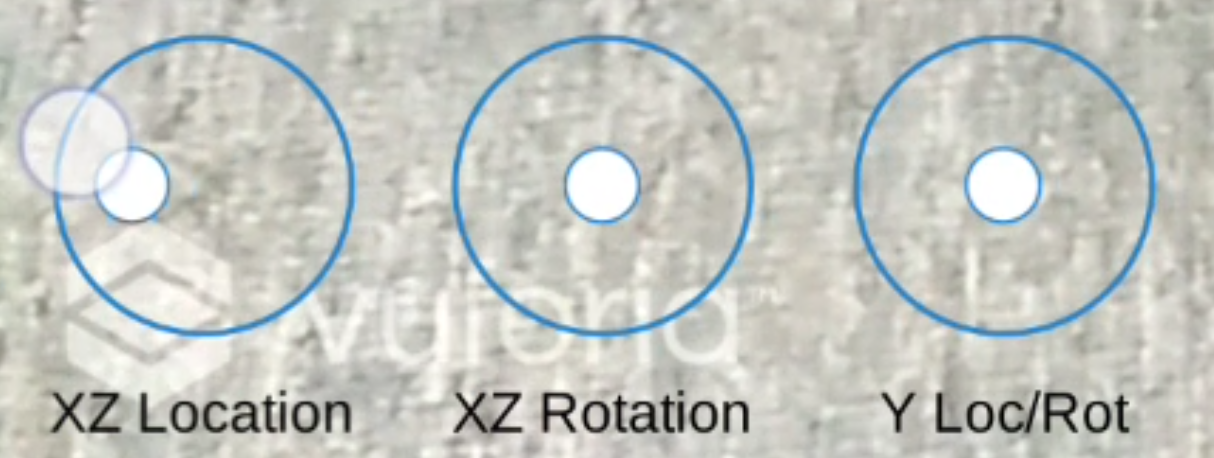
\includegraphics[width=.80\textwidth]{fig/joystick.png}
		\caption{Joystick-like input components.}
		\label{fig:joy}
	\end{figure}
	
	On the right of the scree there are group of and buttons as a menu to control most of logics in this system. The menu contains 4 layers.\ref{fig:menu}
	\begin{itemize}
		\item[(1)] Root layer. Only one button \textit{Building Mode}. It is the entrance of the building mode. By default the system is running in playing mode. Only press the  button can the system enters building mode.
		\item[(2)] Plane layer. Three buttons. \textit{Build Plane \#1} and \textit{Build Plane \#2} are to determine which plane to be edited. \textit{Exit Building Mode} is for exiting building mode (i.e. going into playing mode).
		\item[(3)] Object layer. This layer of buttons are for editing objects placed in a certain plane. All four kinds of objects are included plus a button for define the plane. There are 2 more buttons to make the editing fully functional. \textit{Remove Last Added Object} is for removing the last added object. The added objects are maintained by two separate stacks, each for one plane in the system. \textit{Back to Plane} is for return to the Plane layer menu.
		\item[(4)] \textit{Save Current Object}, \textit{Discard Current Object} and \textit{Save Current Plane} are served for whether to save or discard newly added/defined plane.
	\end{itemize}
	\begin{figure}[htbp]
		\centering
		
\includegraphics[width=.20\textwidth]{fig/m1.png}
		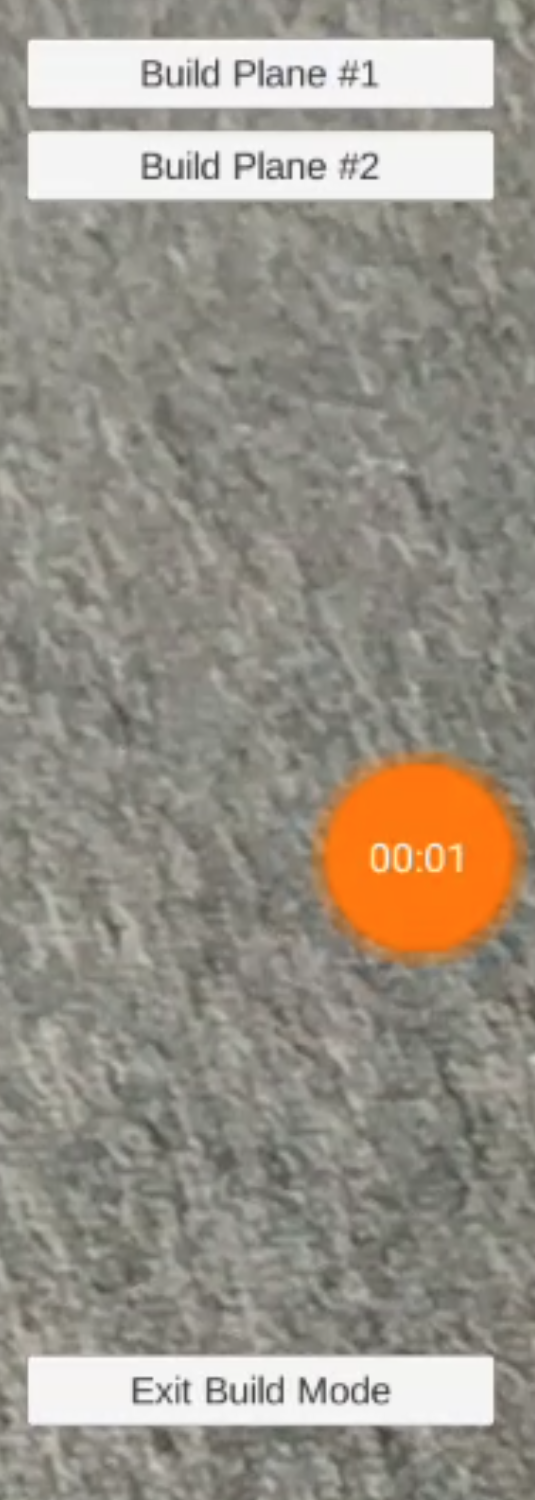
\includegraphics[width=.20\textwidth]{fig/m2.png}
		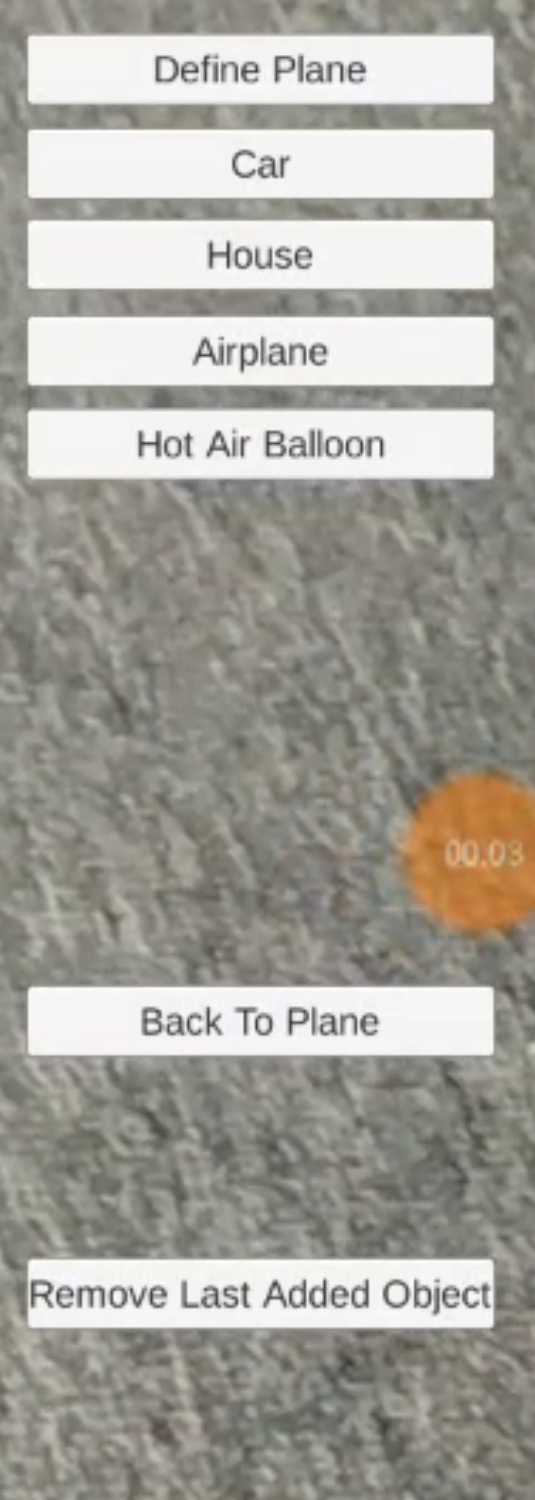
\includegraphics[width=.20\textwidth]{fig/m3.png}
		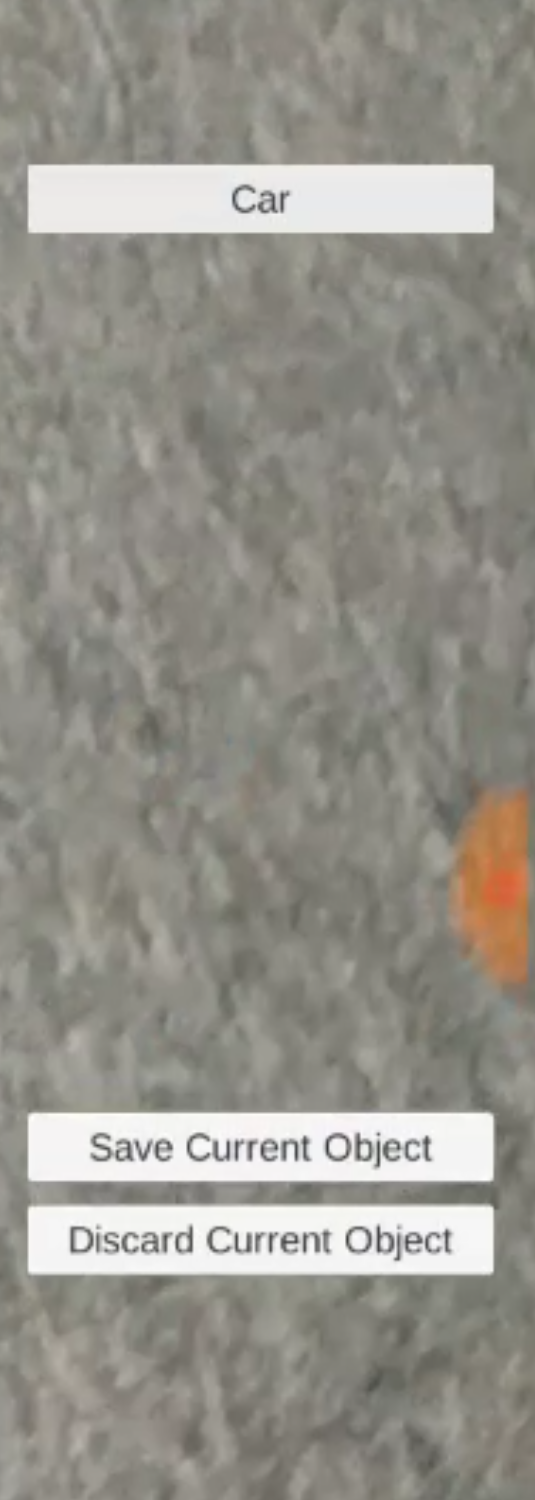
\includegraphics[width=.20\textwidth]{fig/m4.png}
		\caption{Button menu layers.}
		\label{fig:menu}
	\end{figure}
	


	\subsection{Ground Plane Detection}
	Vuforia has its built-in Ground Plane Detection\cite{vuforiagpd} mechanism. However, by default, it places an individual virtual plane in the scene every time the user presses the screen, where the anchor is. In this project, 2 different planes are required, so I develop my own placing method on the top of an open-source piece of code ``DeployStageOnce''.
	
	In the building mode, I design that two planes are defined separately. Hence, within each single plane editing, ``DeployStageOnce'' can be perfectly performed. The only modification I made is moving the part of discriminating duplicated plane placed and placing new anchors to my scene editing codes. Once a specific plane is identified to be editing, it will be initialized at the location of the anchor or translated from the old one to the current one. Old anchors are destroyed to keep the whole scene clean from unused Game Objects.
	
	To illustrate where the plane is placed more obviously, a small cube is placed on the plane. Once a plane is anchored, the cube will give a hint of where the plane is\ref{fig:cube}.
	\begin{figure}[htbp]
		\centering
		
\includegraphics[width=.80\textwidth]{fig/cube.png}
		\caption{Cube identifier.}
		\label{fig:cube}
	\end{figure}

	\subsection{Object Placement}
	The implementation of placing objects can be roughly divided into 3 procedures:
	\begin{itemize}
		\item[(1)] Clone the object from a prefab. This supports dynamically adding objects into the scene, rather than pre-defining several of them.
		\item[(2)] Translate the object to the origin of the corresponding plane.
		\item[(3)] Waiting for user's input to adjust the object's location and rotation. The operation mechanism is described in the part of UI Control\ref{UIC}.
	\end{itemize}
	After these procedures, the user can decide whether to discard or save the object. Once saving, the object can be viewed as settled down on the specific plane, and it will be added into the corresponding stack for further tracking (e.g. remove that object). 
	
	\subsection{Object Motion}
	Cars, planes and hot air balloons are required to move along a certain routine. I directly copy my implementation in Assignment 1 with modification of some speed coefficients to accommodate the coordinator system in this AR environment.
	
	\subsection{Shadow}
	I follow the \cite{arshadow} to allow shadow casting (roughly) correctly in the AR scene. The mechanism is creating a quad on the plane who receives shadows from other objects by a special shader and material.
	\begin{figure}[htbp]
		\centering
		
\includegraphics[width=.80\textwidth]{fig/shadow.png}
		\caption{Shadow.}
		\label{fig:shadow}
	\end{figure}
	\subsection{Day \& Night}
	I implement the day/night mode switching by a check box. The method coded is changing the intensity of the directional light in the day mode from 2 to 0.1 in the night mode. However, it shows no obvious different in real demo.
	
	
	
	
	
	\section{Acknowledgment}
	I would like to thank Xueying Bai and Ying Lu for discussions during this assignment. I also appreciate all the authors of free assets available in the Unity Asset Store.
	%\section{Findings and Results}
	%	Results are shown right in the figures, next to the figure.
	%	\begin{figure}[htbp]
	%		\centering
	%		\includegraphics[width=.90\textwidth]{fig/reselbow.png}
	%		\caption{Elbow Plot}
	%	\end{figure}
	%	\begin{figure}[htbp]
	%		\centering
	%		\includegraphics[width=.90\textwidth]{fig/resscree.png}
	%		\caption{Scree Plot}
	%	\end{figure}
	\bibliography{lab3}
	\bibliographystyle{IEEEtran}
\end{document}


